\chapter{Методология обучения физически-информированной нейронной сети}
С точки зрения машинного обучения и нейронных сетей есть множество важных аспектов,
помимо точности. В контексте физически-информированных нейронных сетей речь пойдет
об оптимизации архитектуры нейронной сети для ускорения обучения, увеличения точности
для оценки компонент скоростей или давления \cite{Tommaso2024pinn}.

Нейронные сети весьма непредсказуемы при обучении, особенно в случае отсутствия
обучающих и тестовых данных. Для понимания работы нейронных сетей в таком режиме
следует изучить влияние количества нейронов, активационной функции и количества слоев,
а также обратить внимание на функции активации, которые определяют,
как нейрон будет реагировать на входные данные, что может существенно влиять на способность
сети обучаться сложным функциям и обобщать полученные данные.
\section{Постановка задачи}
В основе исследуемых задач будем использовать уравнения Навье-Стокса по следующим
причинам:
\begin{enumerate}
    \item Данные уравнения используют частные производные первого и второго порядка
    \item Подразумевается система трех уравнений для двумерной задачи
    \item Наличие трех входных и трех выходных переменных для двумерной задачи
\end{enumerate}
Такой подход позволит рассмотреть физически-информированные нейронные сети на сложных,
с точки зрения модели, задачах, тем самым изучив поведение модели в нетривиальных случаях.

Для анализа будет рассмотрено течение Куэтта в силу его простоты, наличия аналитического
решения, а также наличие нулевого решение для $u_y$ и $p$, что усложняет работу нейронной
сети.
\begin{figure}[ht]
    \caption{Постановка задачи течения Куэтта}
    \label{act_func_graph}
    \centering
    \begin{tikzpicture}[]

        % Размеры
        \def\L{6}   % длина пластин
        \def\H{2}   % расстояние между пластинами
        
        % Пластины
        \draw[thick] (0,0) -- (\L,0); % нижняя пластина
        \draw[thick] (0,\H) -- (\L,\H); % верхняя пластина
        
        % Подписи пластин
        \node[below] at (\L/2,0) {Нижняя пластина (неподвижна)};
        \node[above] at (\L/2,\H) {Верхняя пластина ($U$)};
        
        % Стрелка скорости верхней пластины
        \draw[->,thick,blue] (\L*0.75,\H+0.2) -- (\L*0.75+1,\H+0.2) node[right] {$U$};
        
        % Жидкость между пластинами
        \fill[blue!10] (0,0) rectangle (\L,\H);
        
        % Координаты
        \draw[->] (-0.5,0) -- (-0.5,\H+0.5) node[above] {$y$};
        \draw[->] (-0.5,0) -- (\L+0.5,0) node[right] {$x$};
        
        % Граничные условия
        \draw[->,thick,red] (0.5,0.2) -- (0.5,0.8);
        \node[right,red] at (0.5,0.5) {$u=0$};
        
        \draw[->,thick,red] (0.5,\H-0.2) -- (0.5,\H-0.8);
        \node[right,red] at (0.5,\H-0.5) {$u=U$};
        
        % Подпись слоя жидкости
        \node at (\L/2,\H/2) {Жидкость};
        
        \end{tikzpicture}
    
\end{figure}
Течение Куэтта представляет собой двумерный плоский канал шириной $l$, одна из стенок которого 
движется со скоростью $u_0$. Данная задача имеет аналитическое решение:
\begin{equation}
    \begin{cases}
        u_x = u_0 \frac{y}{l} \\
        u_y = 0 \\
        p = const
    \end{cases}
\end{equation}
где $y$ --- расстояние от неподвижной стенки.

\begin{figure}[ht]
    \caption{}
    \label{points}
    \centering
    \resizebox{0.8\columnwidth}{!}{
        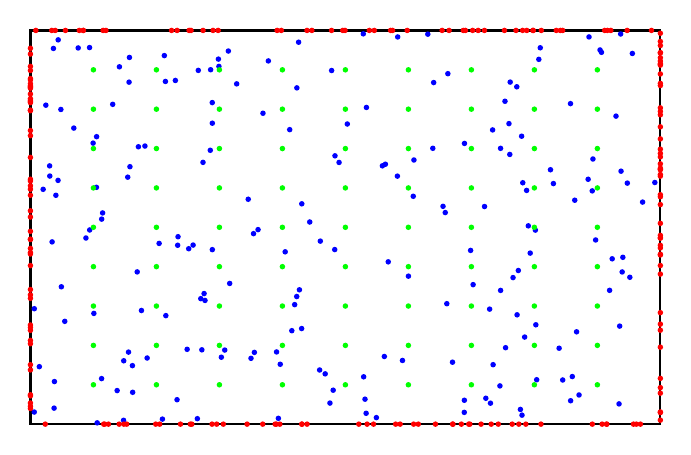
\begin{tikzpicture}
            % Прямоугольник  (размеры 8x5)
            \draw[thick] (-4,-2.5) rectangle (4,2.5);

            % Случайные точки внутри прямоугольника
            \foreach \i in {1,...,200} {
                \fill[blue] (rand*4, rand*2.5) circle (1pt);
            }

            % Случайные точки на гранях прямоугольника
            \foreach \i in {1,...,50} {
                % Нижняя грань
                \fill[red] (rand*4, -2.5) circle (1pt);
                % Верхняя грань
                \fill[red] (rand*4, 2.5) circle (1pt);
                % Левая грань
                \fill[red] (-4, rand*2.5) circle (1pt);
                % Правая грань
                \fill[red] (4, rand*2.5) circle (1pt);
            }

            \foreach \i in {-4,...,4} {
                \foreach \j in {-4,...,4} {
                    \fill[green] (4 * \i / 5, 2.5  * \j / 5) circle (1pt);
                }
            }
        \end{tikzpicture}
        }
    \end{figure}

Используя данное аналитическое решение можно валидировать результаты нейронной сети.

Распределение точек для обучения выглядит примерно следующим образом
(рис. \ref{fig:points}) в каждый момент времени. На каждом временном шаге генерируются случайным
образом набор красных точек на границе и синих точек внутри области. Зеленые точки создаются на 
основе сетки численного (или точного) решения поставленной задачи. Такой подход позволяет использовать
синие и красные точки непосредственно для уравнений Навье-Стокса, красные точки для
граничных условий и зеленые для соответствия с точным решением, вычисленным на определенной
сетке. На такую генерацию накладываются следующие ограничения:
\begin{enumerate}
    \item Количество красных точек следует повышать, если модель отдает предпочтение уравнениям Навье-Стокса
    и игнорирует граничные условия, в результате чего получается нулевое решение.
    \item Количество синих точек следует повышать при недостаточно точном поведении жидкости внутри исследуемой
    области.
    \item Количество зеленых точек следует повышать только в случае, если модель не справляется ни прикаких
    условиях и всегда уходит в локальный минимум.
\end{enumerate}
Данные условия следует выносить в гиперпараметры для повышения качества обучения. В качестве упрощения вместо отдельных
параметров можно использовать отношение синих и красных точек в качестве первого параметра и синих и зеленых --- в 
качестве второго. 


\section{Принцип работы нейронной сети}

Искусственная нейронная сеть представляет собой последовательное преобразование
входного вектора $\mathbf{x}$ посредством набора слоёв (рис. \ref{fig:nn_structure}).
Каждый слой вычисляет взвешенную сумму входных значений с последующим применением
функции активации:

\begin{figure}[ht]
    \caption{Структура PINN с использованием функции активации Adaptive Blending Unit\cite{a104fe01d341f235fd80ea98d6a8f35b8110df1d}}
    \label{pinn_structure}
    \centering
    \resizebox{0.8\columnwidth}{!}{
        \begin{tikzpicture}[node distance=1.2cm, thick]

            % Цвета нод
            \definecolor{inputcolor}{RGB}{255,230,230}   % светло-розовый
            \definecolor{hiddencolor}{RGB}{200,220,255}  % светло-голубой
            \definecolor{outputcolor}{RGB}{220,255,220}  % светло-зелёный
            
            % Входной слой
            \foreach \i in {1,2,3}
                \node[draw, circle, fill=inputcolor, minimum size=1cm] (I\i) at (0,1.8-\i*1.2) {};
            
            % Скрытый слой 1
            \foreach \i in {1,2,3,4}
                \node[draw, circle, fill=hiddencolor, minimum size=1cm] (Hone\i) at (2.5,2.4-\i*1.2) {};
            
            % Скрытый слой 2
            \foreach \i in {1,2,3,4}
                \node[draw, circle, fill=hiddencolor, minimum size=1cm] (Htwo\i) at (5.5,2.4-\i*1.2) {};
            
            % Выходной слой
            \node[draw, circle, fill=outputcolor, minimum size=1cm] (O) at (8.2,-0.6) {};
            
            % Связи: входной -> скрытый 1
            \foreach \i in {1,2,3}
                \foreach \j in {1,2,3,4}
                    \draw[->] (I\i) -- (Hone\j);
            
            % Связи: скрытый 1 -> скрытый 2
            \foreach \i in {1,2,3,4}
                \foreach \j in {1,2,3,4}
                    \draw[->] (Hone\i) -- (Htwo\j);
            
            % Связи: скрытый 2 -> выходной
            \foreach \i in {1,2,3,4}
                \draw[->] (Htwo\i) -- (O);
            
            % Подписи слоёв
            \node[align=center] at (-0.2,2.8) {Входной\\слой};
            \node[align=center] at (2.5,2.8) {Скрытый\\слой 1};
            \node[align=center] at (5.5,2.8) {Скрытый\\слой 2};
            \node[align=center] at (8.2,2.8) {Выходной\\слой};
        \end{tikzpicture}       
    }
\end{figure}

$$
\mathbf{h}^{(l)} = \sigma^{(l)}\left( \mathbf{W}^{(l)} \mathbf{h}^{(l-1)} + \mathbf{b}^{(l)} \right)
$$

где $\mathbf{h}^{(0)} = \mathbf{x}$, $\mathbf{W}^{(l)}$ - матрица весов $l$-го слоя, $\mathbf{b}^{(l)}$ - смещение (bias), $\sigma^{(l)}$ - функция активации.

Обучение сети заключается в минимизации функции потерь $\mathcal{L}$ по параметрам сети $\theta = \{\mathbf{W}, \mathbf{b}\}$.


\section{Функция активации}
Каждый нейрон в нейронной сети использует функцию активации для преобразования взвешенной
суммы своих входных сигналов в выходной сигнал. Эта функция вносит нелинейность в модель,
что необходимо для обучения сложных зависимостей.

Формула, описывающая данный процесс выглядит следующим образом:

$$y = f(\sum_{i=1}^{n} w_i x_i + b)$$

где $x_i$ — $i$-й входной сигнал нейрона, $w_i$ — вес, связанный с $i$-м входным сигналом, $b$
— смещение нейрона, $f(\cdot)$ — функция активации, $y$ — выходной сигнал нейрона.

Для эффективного использования в PINNs функции активации должны удовлетворять следующим
критериям \cite{0d752c79fb816703274a3d37f85a85689a2a9405}:
\begin{itemize}
    \item функции активации должны быть гладкими и
    непрерывно дифференцируемыми, чтобы обрабатывать функции потерь, которые включают
    производные высших порядков.
    \item функции активации должны допускать неограниченные
    выходные значения, в отличие от функций $tanh$ и $sin$, которые ограничены между $-1$ и $1$.
    \item функции активации должны избегать насыщения, чтобы предотвратить
    исчезновение градиентов, что может затруднить обучение.
    \item в некоторых случаях желательно иметь контролируемое насыщение за пределами определённого
    диапазона, чтобы улучшить способность модели представлять сложные физические сигналы.
\end{itemize}


Функция активации $\sigma(x)$ определяет нелинейность слоя и влияет на способность
сети аппроксимировать сложные зависимости. В данной работе рассмотрены следующие функции
(табл. \ref{table:act_basic}).

\begin{table}[h!]
    \centering
    \caption{Основные функции активации \cite{tensorflow2015-whitepaper}}
    \renewcommand{\arraystretch}{1.5}
    \begin{tabular}{|c|c|p{7cm}|}
    \hline
    \textbf{Функция} & \textbf{Математическая формула} & \textbf{Назначение и свойства} \\
    \hline
    $\tanh$ & $\sigma(x) = \dfrac{e^{x} - e^{-x}}{e^{x} + e^{-x}}$ & Гладкая, нечётная функция с непрерывной производной. \\
    \hline
    $\sin$ & $\sigma(x) = \sin(x)$ & Используется для задач с выраженной периодичностью решения. \\
    \hline
    $\exp$ & $\sigma(x) = \exp(x)$ & Применяется для задач с экспоненциальным затуханием. \\
    \hline
    Сигмоида & $\sigma(x) = \dfrac{1}{1 + e^{-x}}$ & Гладкая функция, полезная для нормализации выходных значений. \\
    \hline
    Квадратичная & $\sigma(x) = \dfrac{1}{1 + x^2}$ & Гладкая функция с ограниченным выходом, не монотонна. \\
    \hline
    Softplus & $\sigma(x) = \log(1 + \exp(x))$ & Плавная аппроксимация ReLU, дифференцируемая и монотонная. \\
    \hline
    SiLU & $\sigma(x) = x * \sigma(x)$ & Сглаженная версия ReLU, улучшает обучение глубоких сетей. \\
    \hline
    \end{tabular}
    \label{table:act_basic}
\end{table}

\section{Оптимизаторы}
В процессе обучения нейронной сети для минимизации функции потерь $\mathcal{L}(\theta)$ по параметрам $\theta$ используются различные оптимизаторы. Ниже приведены основные из них:

\begin{itemize}
    \item \textbf{Adam}~\cite{kingma2014adam} --- адаптивный метод, основанный на оценке первых и вторых моментов градиентов. На каждой итерации параметры обновляются по правилу:
    \[
    \begin{aligned}
        m_t &= \beta_1 m_{t-1} + (1 - \beta_1) g_t \\
        v_t &= \beta_2 v_{t-1} + (1 - \beta_2) g_t^2 \\
        \hat{m}_t &= \frac{m_t}{1 - \beta_1^t} \\
        \hat{v}_t &= \frac{v_t}{1 - \beta_2^t} \\
        \theta_{t+1} &= \theta_t - \eta \frac{\hat{m}_t}{\sqrt{\hat{v}_t} + \epsilon}
    \end{aligned}
    \]
    где $g_t$ --- градиент на шаге $t$, $\eta$ --- скорость обучения, $\beta_1$, $\beta_2$ --- параметры экспоненциального сглаживания, $\epsilon$ --- малая константа для избежания деления на ноль.

    \item \textbf{Adagrad}~\cite{duchi2011adaptive} --- оптимизатор, индивидуально адаптирующий скорость обучения для каждого параметра:
    \[
    \begin{aligned}
        G_t &= G_{t-1} + g_t^2 \\
        \theta_{t+1} &= \theta_t - \frac{\eta}{\sqrt{G_t} + \epsilon} g_t
    \end{aligned}
    \]
    где $G_t$ --- накопленная сумма квадратов градиентов.

    \item \textbf{Adamax}~\cite{kingma2014adam} --- вариант Adam, использующий норму $L_\infty$ вместо $L_2$ для второго момента:
    \[
    \begin{aligned}
        m_t &= \beta_1 m_{t-1} + (1 - \beta_1) g_t \\
        u_t &= \max(\beta_2 u_{t-1}, |g_t|) \\
        \theta_{t+1} &= \theta_t - \frac{\eta}{u_t} m_t
    \end{aligned}
    \]
    Обеспечивает устойчивость при больших градиентах.

    \item \textbf{ASGD} (Averaged Stochastic Gradient Descent)~\cite{polyak1992acceleration} --- стохастический градиентный спуск с усреднением параметров:
    \[
    \begin{aligned}
        \theta_{t+1} &= \theta_t - \eta g_t \\
        \bar{\theta}_t &= \frac{1}{t} \sum_{k=1}^{t} \theta_k
    \end{aligned}
    \]
    где $\bar{\theta}_t$ --- усреднённые параметры, что способствует лучшей сходимости и устойчивости.

    \item \textbf{RMSprop}~\cite{tieleman2012lecture} --- оптимизатор, который нормирует градиент с помощью скользящего среднего квадратов градиентов:
    \[
    \begin{aligned}
        E[g^2]_t &= \gamma E[g^2]_{t-1} + (1 - \gamma) g_t^2 \\
        \theta_{t+1} &= \theta_t - \frac{\eta}{\sqrt{E[g^2]_t} + \epsilon} g_t
    \end{aligned}
    \]
    где $\gamma$ --- коэффициент сглаживания.
\end{itemize}

\section{Процесс обучения}
Обучение проводилось с использованием фреймворка PyTorch, а также вспомогательных
библиотек и утилит tensorboard и ray tune.

Для повышения качества результатов и значительного сокращения времени вычислений и
исследований, кросс-валидация гиперпараметров модели будет проведена в два
последовательных этапа.

Вначале применяется адаптивная функция активации
REAct~\cite{0d752c79fb816703274a3d37f85a85689a2a9405}, обусловленная её вычислительной
простотой и высокой скоростью оценки значений и производных, что существенно
повышает эффективность проведения кросс-валидации. Поскольку теоретически
невозможно предсказать поведение модели при различных параметрических настройках,
кросс-валидация реализуется посредством метода перебора по сетке. В качестве
гиперпараметров рассматриваются конфигурация нейронной сети, выбор оптимизатора,
функция активации, количество точек внутри области, а также скорость обучения.


Архитектура нейронной сети исследуется с применением вариативного подхода к
подбору количества и конфигурации слоев, охватывающего как компактные структуры
(например, $16-16$ и $32-32$), так и более глубокие многослойные комбинации,
включая $32-64-32$, $64-32-64$, а также асимметричные схемы, такие как
$16-32-64$, $64-32-16$, $16-64-32$ и $64-16-32$. Особое внимание уделяется
масштабируемым конфигурациям, например $64-64$, с целью оценки влияния
вариаций числа нейронов на эффективность модели. Такой подход позволяет
систематически анализировать зависимость производительности нейронной сети
от структуры и глубины архитектуры, что является ключевым аспектом при
оптимизации моделей машинного обучения.

Для изучения влияния выбора оптимизатора на качество результатов были выбраны
следующие алгоритмы оптимизации: \textbf{Adam}, \textbf{Adagrad}, \textbf{Adamax},
а также специализированные методы \textbf{ASGD} и \textbf{RMSprop}.

Для анализа влияния параметров функции активации была выбрана группа из четырёх вариаций параметров
REAct с различными параметрическими настройками (см. рис. \ref{fig:react_func_graph}).
\begin{figure}[ht]
    \caption{Функции активации на основе REAct}
    \label{act_func_graph}
    \centering
    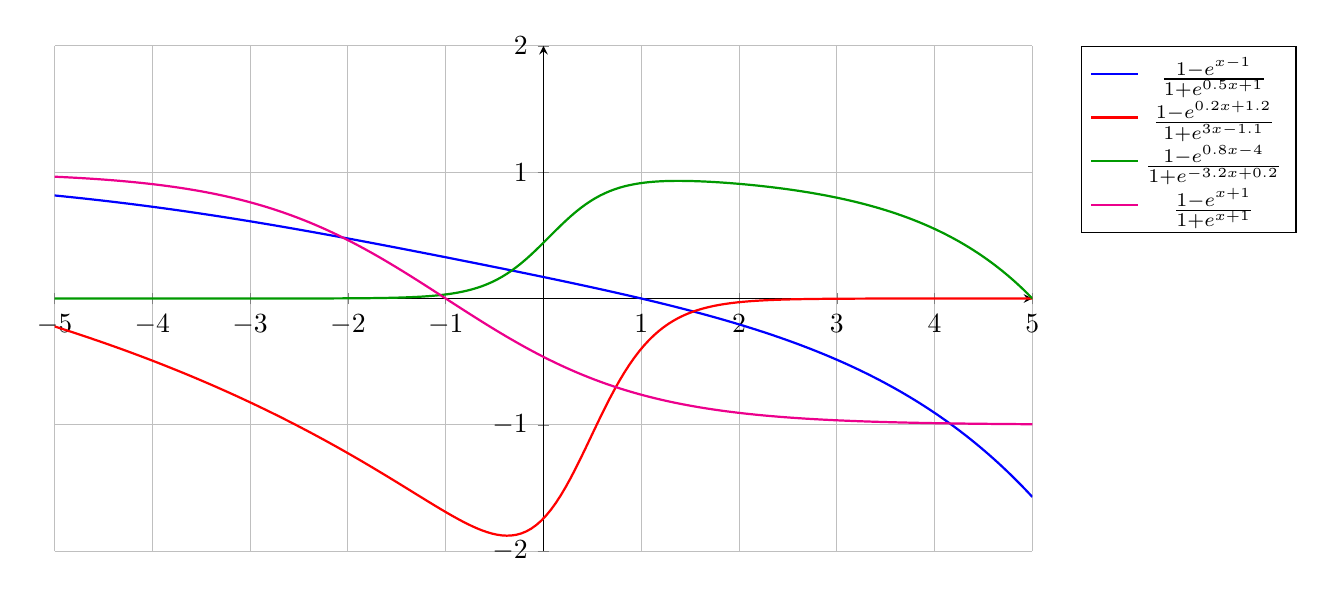
\begin{tikzpicture}
        \begin{axis}[
            width=14cm,
            height=8cm,
            xmin=-5, xmax=5,
            ymin=-2, ymax=2,
            axis lines=middle,
            grid=both,
            legend style={at={(1.05,1)},anchor=north west}
        ]
        % 1. [1, -1, 0.5, 1]
        \addplot[
            domain=-5:5, 
            samples=200, 
            thick, 
            blue
        ]
        {(1 - exp(1*x - 1)) / (1 + exp(0.5*x + 1))};
        \addlegendentry{$\frac{1 - e^{x - 1}}{1 + e^{0.5x + 1}}$}
        
        % 2. [0.2, 1.2, 3, -1.1]
        \addplot[
            domain=-5:5, 
            samples=200, 
            thick, 
            red
        ]
        {(1 - exp(0.2*x + 1.2)) / (1 + exp(3*x - 1.1))};
        \addlegendentry{$\frac{1 - e^{0.2x + 1.2}}{1 + e^{3x - 1.1}}$}
        
        % 3. [0.8, -4, -3.2, 0.2]
        \addplot[
            domain=-5:5, 
            samples=200, 
            thick, 
            green!60!black
        ]
        {(1 - exp(0.8*x - 4)) / (1 + exp(-3.2*x + 0.2))};
        \addlegendentry{$\frac{1 - e^{0.8x - 4}}{1 + e^{-3.2x + 0.2}}$}
        
        % 4. [1, 1, 1, 1]
        \addplot[
            domain=-5:5, 
            samples=200, 
            thick, 
            magenta
        ]
        {(1 - exp(1*x + 1)) / (1 + exp(1*x + 1))};
        \addlegendentry{$\frac{1 - e^{x + 1}}{1 + e^{x + 1}}$}
        
        \end{axis}
    \end{tikzpicture}
    
\end{figure}

Обучающая выборка варьировалась между $100$ и $500$ точками для внутренней
области и неизменных $1000$ точек для граничных условий. 

Скорость обучения задавалась тремя значениями: $10^{-1}$, $10^{-2}$ и $10^{-3}$.

По итогам первого этапа исследования производится отбор наиболее эффективных результатов,
на основании которых осуществляется исключение неподходящих параметров модели.

\begin{figure}[ht]
    \caption{Функции активации на основе REAct}
    \label{fig:abu_func_graph}
    \centering
    \begin{tikzpicture}
        \begin{axis}[
            width=16cm,
            height=10cm,
            xmin=-4, xmax=4,
            ymin=-3, ymax=8,
            axis lines=middle,
            grid=both,
            legend style={at={(1.05,1)},anchor=north west, font=\footnotesize},
            cycle list name=color list,
            samples=200
        ]
        
        % Функция swish(x) = x * sigmoid(x)
        \pgfmathdeclarefunction{swish}{1}{
          \pgfmathparse{#1/(1+exp(-#1))}
        }
        
        % Функция softplus(x) = ln(1 + exp(x))
        \pgfmathdeclarefunction{softplus}{1}{
          \pgfmathparse{ln(1 + exp(#1))}
        }
        
        % Перебор всех комбинаций (a, b, c, d)
        \foreach \a/\b/\c/\d in {0/0/0/0, 0/0/0/1, 0/0/1/0, 0/0/1/1,
                                 0/1/0/0, 0/1/0/1, 0/1/1/0, 0/1/1/1,
                                 1/0/0/0, 1/0/0/1, 1/0/1/0, 1/0/1/1,
                                 1/1/0/0, 1/1/0/1, 1/1/1/0, 1/1/1/1}
        {
            \addplot+[thick] 
            ({x},
             {sin(deg(x)) 
              + (\a == 1 ? tanh(x) : 0)
              + (\b == 1 ? swish(x) : 0)
              + (\c == 1 ? 1/(1 + x^2) : 1)
              + (\d == 1 ? softplus(x) : 0)
             });
            % \addlegendentry{$a=\a,\,b=\b,\,c=\c,\,d=\d$}
        }
        
        \end{axis}
    \end{tikzpicture}
    
\end{figure}

На втором этапе обучения используется комплексная функция активации
\textbf{ABU}~\cite{Sutfeld2018-io}, что позволяет повысить адаптивность модели за счёт
комбинирования различных активационных механизмов.

В рамках исследования, в качестве функций $\sigma_i$, входящих в уравнение \eqref{eq:abu},
используются $\mathbf{sin}$, $\mathbf{tanh}$, $\mathbf{SiLU}$, $\mathbf{quadratic}$ и
$\mathbf{softplus}$. Коэффициенты для кроссвалидации принимают значения $0$ или $1$ для всех
функций, за исключением $\mathbf{sin}$. Графическое представление данных функций приведено
на рис. \ref{fig:abu_func_graph}.
Другими словами функция активации имеет следующий вид:
\begin{equation}
    \begin{split}
        \text{ABU}(x) = \sin(x) &+ \text{Quadratic}(\beta_0 x) + \\
        &+ \text{Softplus}(\beta_1 x) + \text{SiLU}(\beta_2 x) + \tanh(\beta_3 x),
    \end{split}
    \label{eq:abu_custom}
\end{equation}
где $\beta_i$ --- коэффициент для кроссвалидации,  принимающий значения $0$ или $1$.


Для обеспечения более точной оценки результатов проводится анализ медианных значений каждого
параметра на протяжении всего периода обучения.